\documentclass[tikz, border=6pt]{standalone}
\usepackage[T1]{fontenc}
\usepackage{lmodern}
\usepackage{amsmath,amssymb,bm}
\usepackage[scaled=0.95]{helvet}
\usetikzlibrary{arrows.meta}
\definecolor{Blue}{HTML}{3A76D8}
\definecolor{Green}{HTML}{3BA55C}
\definecolor{Orange}{HTML}{EE8133}
\definecolor{Red}{HTML}{DF4B4B}
\definecolor{Gray}{HTML}{6B7280}
\definecolor{Ink}{HTML}{1F2937}
\definecolor{cC0C3C7}{HTML}{C0C3C7}
\definecolor{cD7D8DB}{HTML}{D7D8DB}
\definecolor{cE8E9EB}{HTML}{E8E9EB}
\definecolor{cFBFBFB}{HTML}{FBFBFB}
\definecolor{cE1E2E4}{HTML}{E1E2E4}
\definecolor{c626973}{HTML}{626973}
\definecolor{c5E656F}{HTML}{5E656F}
\definecolor{cFBFCFC}{HTML}{FBFCFC}
\definecolor{cB1B4B9}{HTML}{B1B4B9}
\definecolor{cCCCED2}{HTML}{CCCED2}
\definecolor{cEDEDEF}{HTML}{EDEDEF}
\definecolor{c404955}{HTML}{404955}
\definecolor{cB3B6BB}{HTML}{B3B6BB}
\definecolor{cB9BCC0}{HTML}{B9BCC0}
\definecolor{cBDC0C4}{HTML}{BDC0C4}
\definecolor{c636A73}{HTML}{636A73}
\definecolor{c3B4450}{HTML}{3B4450}
\definecolor{c4D5560}{HTML}{4D5560}
\definecolor{cD3D5D8}{HTML}{D3D5D8}
\definecolor{cEAEBEC}{HTML}{EAEBEC}
\definecolor{cBABDC1}{HTML}{BABDC1}
\definecolor{cFAFAFA}{HTML}{FAFAFA}
\definecolor{cC9CCCF}{HTML}{C9CCCF}
\definecolor{cFFFFFF}{HTML}{FFFFFF}
\definecolor{c4C545F}{HTML}{4C545F}
\definecolor{c1F2937}{HTML}{1F2937}
\definecolor{cECECEC}{HTML}{ECECEC}
\definecolor{cA5A5A5}{HTML}{A5A5A5}
\definecolor{cB2B2B2}{HTML}{B2B2B2}
\definecolor{cD4D4D4}{HTML}{D4D4D4}
\definecolor{cC4C4C4}{HTML}{C4C4C4}
\definecolor{c707070}{HTML}{707070}
\tikzset{
  block/.style={/utils/exec={\colorlet{pytikzarg}{#1}}, draw=pytikzarg!78!black, fill=pytikzarg!14, rounded corners=3pt, align=center, inner sep=5pt, minimum height=8mm, minimum width=20mm},
  block/.default=Blue,
}
\begin{document}
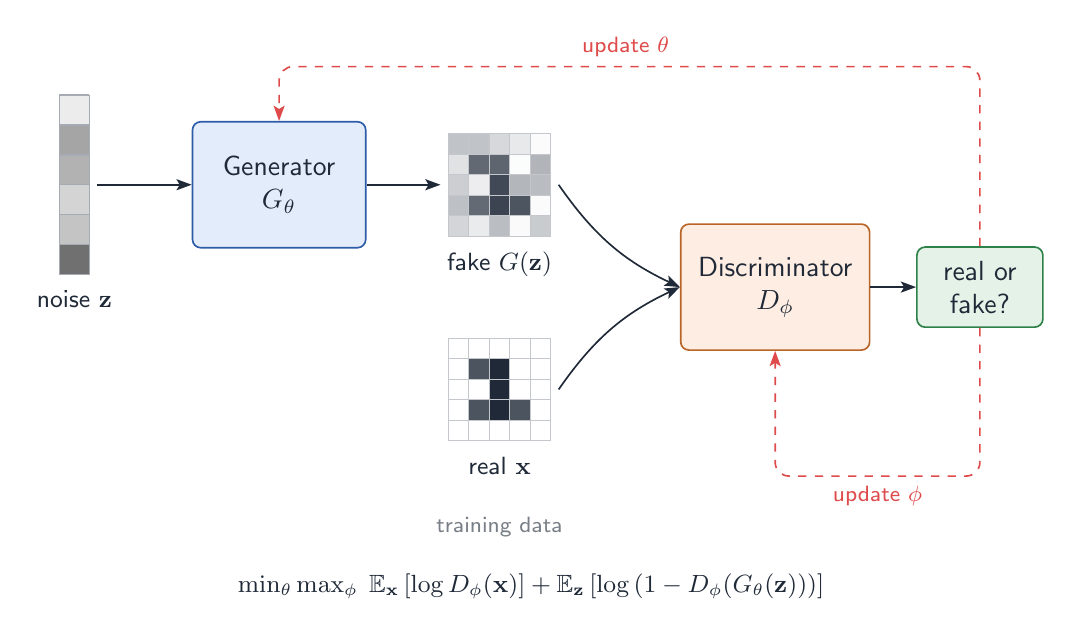
\begin{tikzpicture}[color=Ink, execute at begin picture={\sffamily}, line width=0.6pt, >={Stealth[length=5.5pt, width=4pt, inset=1.2pt]}, line join=round]
  % cell grid  6x1
  \fill[cECECEC] (-0.19,2.36) rectangle (0.19,2.74);
  \fill[cA5A5A5] (-0.19,1.98) rectangle (0.19,2.36);
  \fill[cB2B2B2] (-0.19,1.6) rectangle (0.19,1.98);
  \fill[cD4D4D4] (-0.19,1.22) rectangle (0.19,1.6);
  \fill[cC4C4C4] (-0.19,0.84) rectangle (0.19,1.22);
  \fill[c707070] (-0.19,0.46) rectangle (0.19,0.84);
  \draw[Gray!60, line width=0.5pt] (-0.19,0.46) -- (0.19,0.46) (-0.19,0.84) -- (0.19,0.84) (-0.19,1.22) -- (0.19,1.22) (-0.19,1.6) -- (0.19,1.6) (-0.19,1.98) -- (0.19,1.98) (-0.19,2.36) -- (0.19,2.36) (-0.19,2.74) -- (0.19,2.74) (-0.19,0.46) -- (-0.19,2.74) (0.19,0.46) -- (0.19,2.74);
  \node[anchor=north, font=\small, align=center] at (0,0.38) {noise $\mathbf{z}$};
  \node[align=center, block=Blue, minimum width=2.2cm, minimum height=1.6cm] (n1) at (2.6,1.6) {Generator\\$G_\theta$};
  \draw[->] (0.29,1.6) -- (n1);
  % cell grid  5x5
  \fill[cC0C3C7] (4.75,1.99) rectangle (5.01,2.25) (5.01,1.99) rectangle (5.27,2.25);
  \fill[cD7D8DB] (5.27,1.99) rectangle (5.53,2.25);
  \fill[cE8E9EB] (5.53,1.99) rectangle (5.79,2.25);
  \fill[cFBFBFB] (5.79,1.99) rectangle (6.05,2.25) (5.79,1.21) rectangle (6.05,1.47);
  \fill[cE1E2E4] (4.75,1.73) rectangle (5.01,1.99);
  \fill[c626973] (5.01,1.73) rectangle (5.27,1.99);
  \fill[c5E656F] (5.27,1.73) rectangle (5.53,1.99);
  \fill[cFBFCFC] (5.53,1.73) rectangle (5.79,1.99);
  \fill[cB1B4B9] (5.79,1.73) rectangle (6.05,1.99);
  \fill[cCCCED2] (4.75,1.47) rectangle (5.01,1.73);
  \fill[cEDEDEF] (5.01,1.47) rectangle (5.27,1.73);
  \fill[c404955] (5.27,1.47) rectangle (5.53,1.73);
  \fill[cB3B6BB] (5.53,1.47) rectangle (5.79,1.73);
  \fill[cB9BCC0] (5.79,1.47) rectangle (6.05,1.73);
  \fill[cBDC0C4] (4.75,1.21) rectangle (5.01,1.47);
  \fill[c636A73] (5.01,1.21) rectangle (5.27,1.47);
  \fill[c3B4450] (5.27,1.21) rectangle (5.53,1.47);
  \fill[c4D5560] (5.53,1.21) rectangle (5.79,1.47);
  \fill[cD3D5D8] (4.75,0.95) rectangle (5.01,1.21);
  \fill[cEAEBEC] (5.01,0.95) rectangle (5.27,1.21);
  \fill[cBABDC1] (5.27,0.95) rectangle (5.53,1.21);
  \fill[cFAFAFA] (5.53,0.95) rectangle (5.79,1.21);
  \fill[cC9CCCF] (5.79,0.95) rectangle (6.05,1.21);
  \draw[Gray!40, line width=0.3pt] (4.75,0.95) -- (6.05,0.95) (4.75,1.21) -- (6.05,1.21) (4.75,1.47) -- (6.05,1.47) (4.75,1.73) -- (6.05,1.73) (4.75,1.99) -- (6.05,1.99) (4.75,2.25) -- (6.05,2.25) (4.75,0.95) -- (4.75,2.25) (5.01,0.95) -- (5.01,2.25) (5.27,0.95) -- (5.27,2.25) (5.53,0.95) -- (5.53,2.25) (5.79,0.95) -- (5.79,2.25) (6.05,0.95) -- (6.05,2.25);
  \node[anchor=north, font=\small, align=center] at (5.4,0.87) {fake $G(\mathbf{z})$};
  % cell grid  5x5
  \fill[cFFFFFF] (4.75,-0.61) rectangle (5.01,-0.35) (5.01,-0.61) rectangle (5.27,-0.35) (5.27,-0.61) rectangle (5.53,-0.35) (5.53,-0.61) rectangle (5.79,-0.35) (5.79,-0.61) rectangle (6.05,-0.35) (4.75,-0.87) rectangle (5.01,-0.61) (5.53,-0.87) rectangle (5.79,-0.61) (5.79,-0.87) rectangle (6.05,-0.61) (4.75,-1.13) rectangle (5.01,-0.87) (5.01,-1.13) rectangle (5.27,-0.87) (5.53,-1.13) rectangle (5.79,-0.87) (5.79,-1.13) rectangle (6.05,-0.87) (4.75,-1.39) rectangle (5.01,-1.13) (5.79,-1.39) rectangle (6.05,-1.13) (4.75,-1.65) rectangle (5.01,-1.39) (5.01,-1.65) rectangle (5.27,-1.39) (5.27,-1.65) rectangle (5.53,-1.39) (5.53,-1.65) rectangle (5.79,-1.39) (5.79,-1.65) rectangle (6.05,-1.39);
  \fill[c4C545F] (5.01,-0.87) rectangle (5.27,-0.61) (5.01,-1.39) rectangle (5.27,-1.13) (5.53,-1.39) rectangle (5.79,-1.13);
  \fill[c1F2937] (5.27,-0.87) rectangle (5.53,-0.61) (5.27,-1.13) rectangle (5.53,-0.87) (5.27,-1.39) rectangle (5.53,-1.13);
  \draw[Gray!40, line width=0.3pt] (4.75,-1.65) -- (6.05,-1.65) (4.75,-1.39) -- (6.05,-1.39) (4.75,-1.13) -- (6.05,-1.13) (4.75,-0.87) -- (6.05,-0.87) (4.75,-0.61) -- (6.05,-0.61) (4.75,-0.35) -- (6.05,-0.35) (4.75,-1.65) -- (4.75,-0.35) (5.01,-1.65) -- (5.01,-0.35) (5.27,-1.65) -- (5.27,-0.35) (5.53,-1.65) -- (5.53,-0.35) (5.79,-1.65) -- (5.79,-0.35) (6.05,-1.65) -- (6.05,-0.35);
  \node[anchor=north, font=\small, align=center] at (5.4,-1.73) {real $\mathbf{x}$};
  \draw[->] (n1) -- (4.65,1.6);
  \node[font=\footnotesize, text=Ink!60] at (5.4,-2.75) {training data};
  \node[align=center, block=Orange, minimum width=2.4cm, minimum height=1.6cm] (n2) at (8.9,0.3) {Discriminator\\$D_\phi$};
  \draw[->] (6.15,1.6) to[bend right=15] (n2.west);
  \draw[->] (6.15,-1) to[bend left=15] (n2.west);
  \node[align=center, block=Green, minimum width=1.6cm] (n3) at (11.5,0.3) {real or\\fake?};
  \draw[->] (n2) -- (n3);
  \draw[->, dashed, color=Red, rounded corners=5pt] (n3.south) -- (11.5,-2.1) -- (8.9,-2.1) --
      (n2.south);
  \draw[->, dashed, color=Red, rounded corners=5pt] (n3.north) -- (11.5,3.1) -- (2.6,3.1) --
      (n1.north);
  \node[anchor=north, font=\footnotesize, text=Red] at (10.2,-2.1) {update $\phi$};
  \node[anchor=south, font=\footnotesize, text=Red] at (7,3.1) {update $\theta$};
  \node[font=\small] at (5.8,-3.5) {$\min_\theta \max_\phi \; \mathbb{E}_{\mathbf{x}}\left[\log D_\phi(\mathbf{x})\right] + \mathbb{E}_{\mathbf{z}}\left[\log\left(1 - D_\phi(G_\theta(\mathbf{z}))\right)\right]$};
\end{tikzpicture}
\end{document}
